\chapter{SYSTEM ARCHITECTURE AND METHODOLOGY}



\section{System Block Diagram}

\begin{figure}[H]
\centering
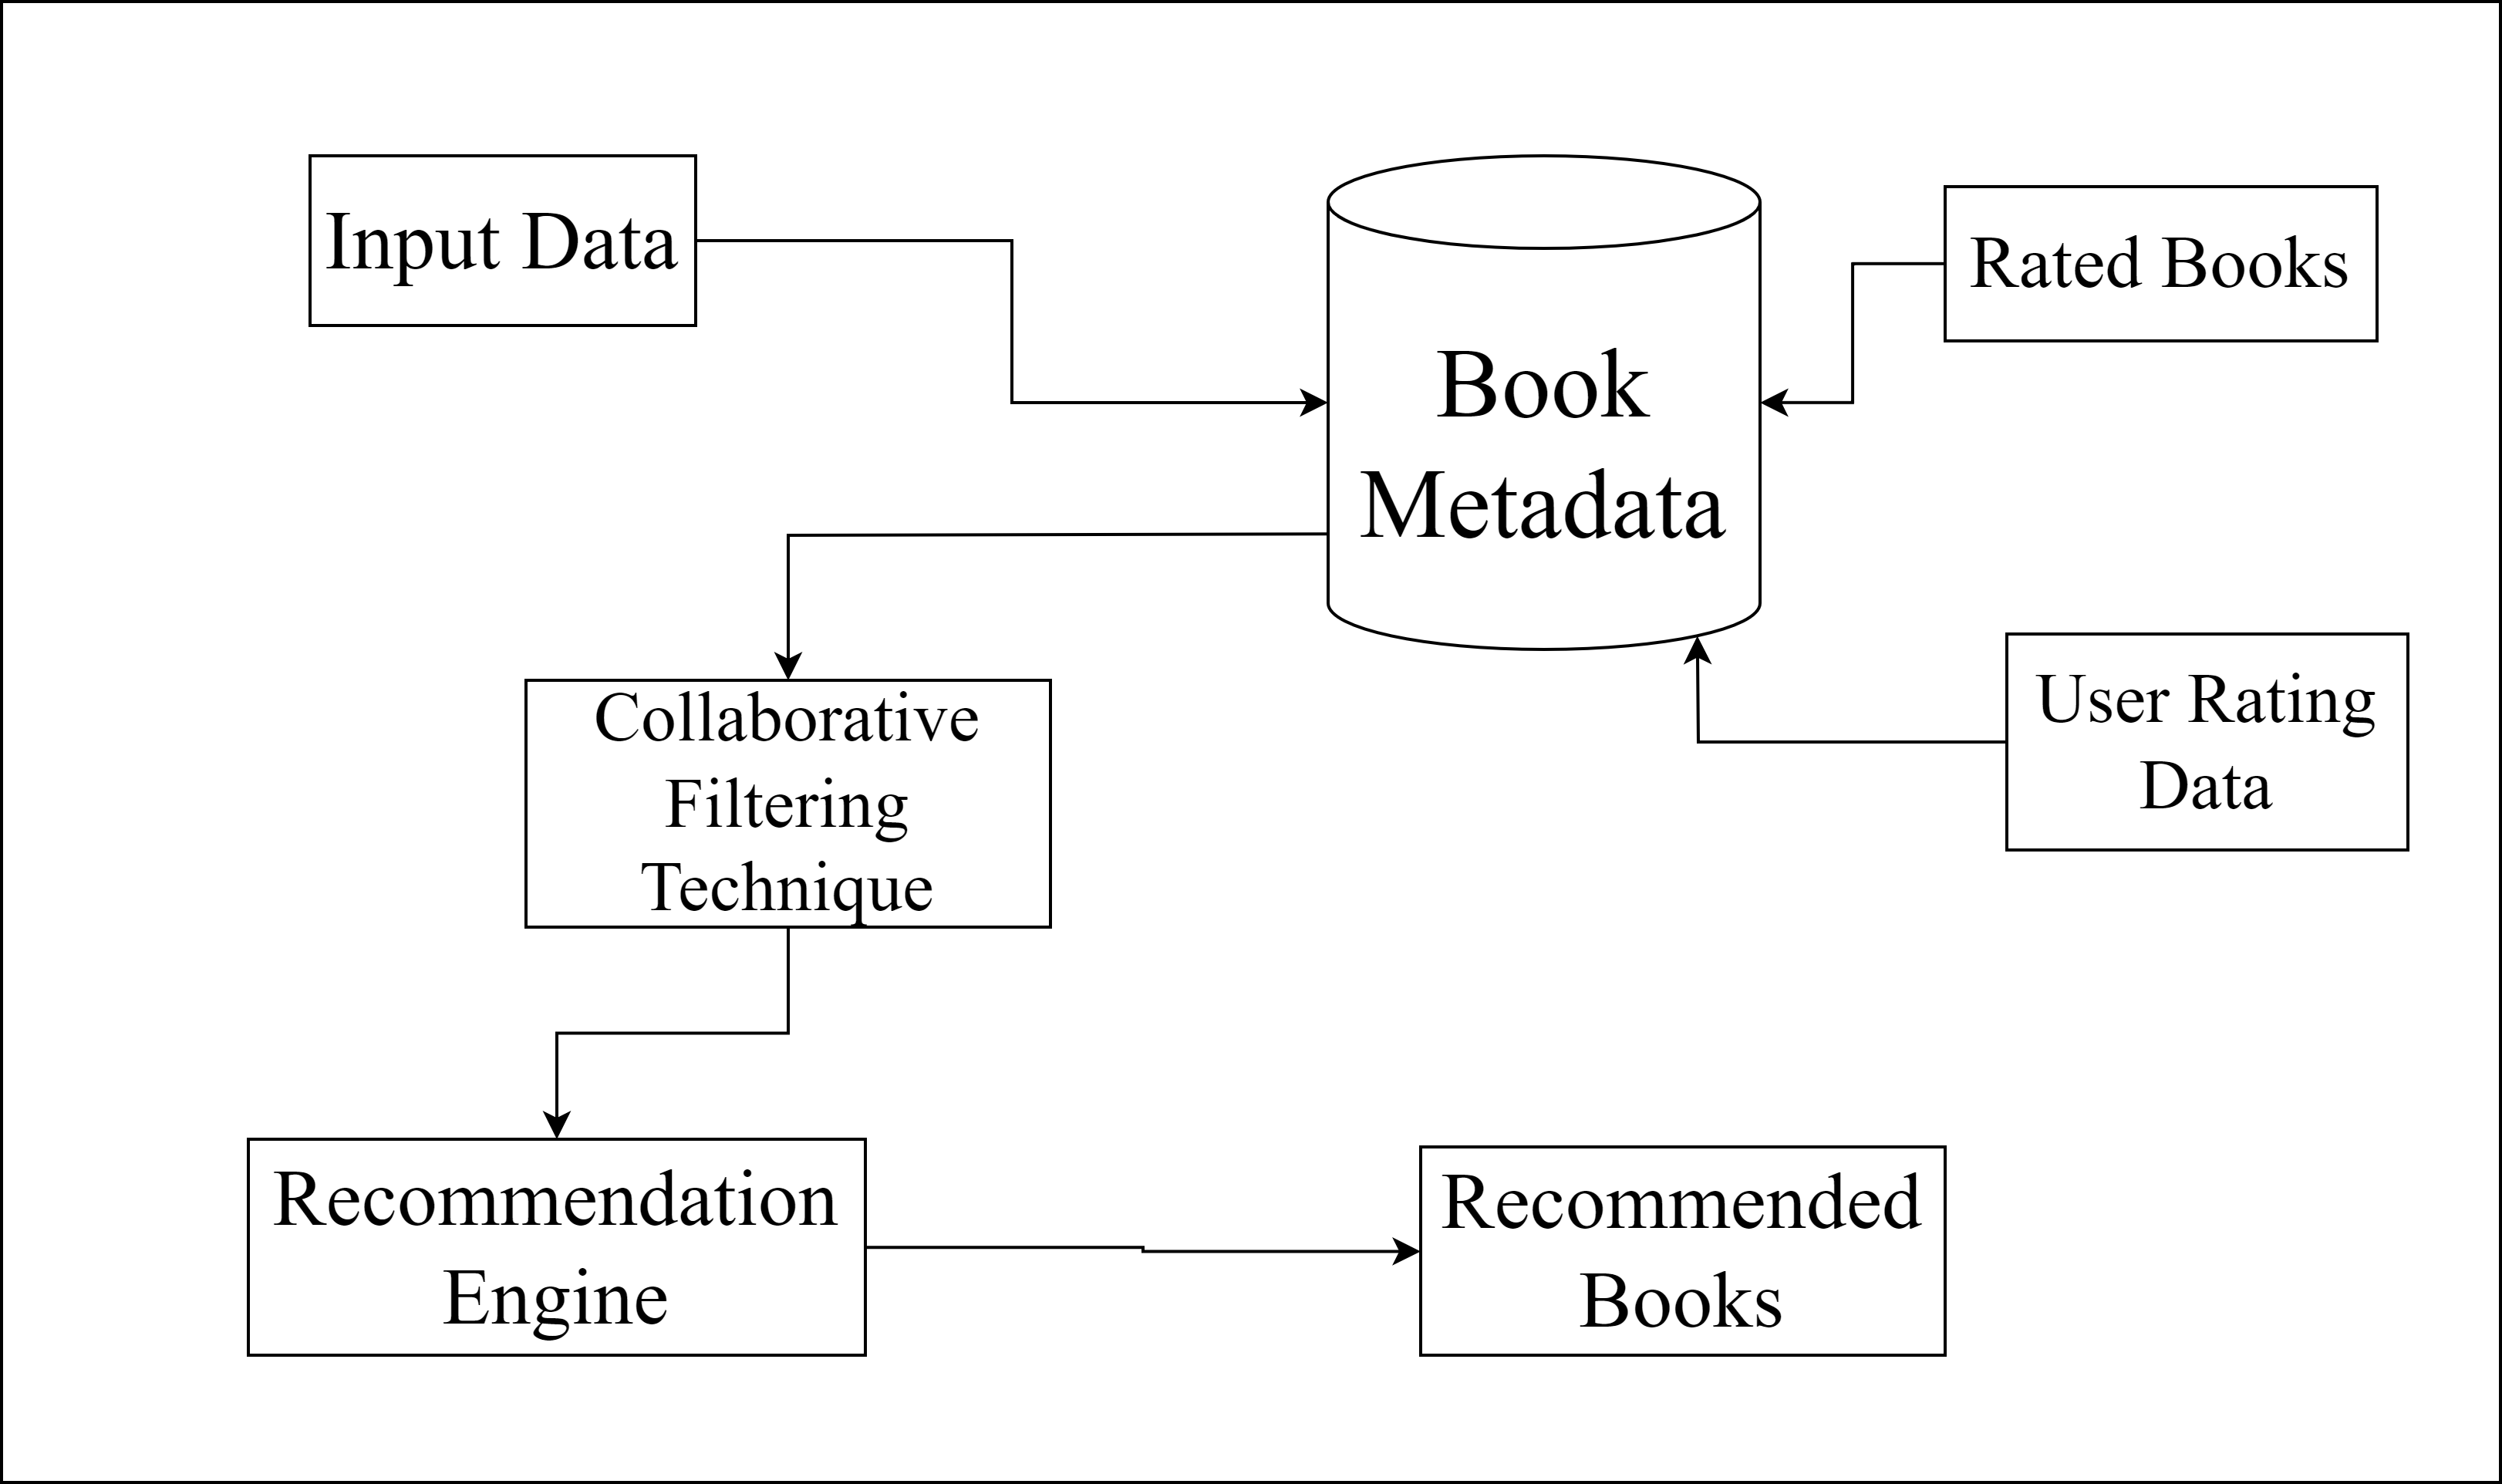
\includegraphics[width=0.8\linewidth]{img/Graphics/BRS_block_Diagram.drawio.png}
\caption[System Block Diagram]{System Block Diagram}
\label{fig:SystemBlockDiagram.png}

\end{figure} 
    \subsection{Input Data}
    In the book recommendation system, book name is entered in the user interface as input data. The input data is transferred into the recommendation engine for processing through user interface. Users can express their tastes and interests through the input data, which acts as the basis for the recommendation process.
    \subsection{Book Metadata}  
    This is the database that contains the information about the books available in the system. It will include name of the book, ISBN, publisher, cover images, author(s), year of publication and genre. Book metadata is essential for giving users thorough information and enabling precise recommendations.
    \subsection{Collaborative Filtering Technique} 
    This is the recommendation technique for analyzing user data to make personalized recommendations based on patterns found in the preferences and actions of the users. This technique includes KNN-algorithm to find the most similar items and users based on the attributes and particular features for generating tailored recommendations.
    \subsection{Rated Books}  
    The term rated books refers to the collection of data that includes book ratings given to it by different users. This information is crucial for collaborative filtering because it makes user preferences and behaviours easier to understand. The recommendation system can produce more accurate recommendations by identifying trends and similarities among users through the analysis of rated books.  
    \subsection{User Rating Data} 
    The ratings that different users have assigned to particular books make up the user rating data. This information is essential for collaborative filtering algorithms because it provides light on user preferences and helps assess how relevant a given item is to a given user. The user rating data is utilized to provide tailored recommendations.
    \subsection{Recommendation Engine}
    This is the key component of the system that generates the recommendation of the books. It generates a personalised book recommendation list for each user based on collaborative filtering techniques. For this system the engine is based on KNN model. It may includes others factors such as trending books, popular books.
    \subsection{Recommended Books}
    The list of books generated by the recommendation engine based on the taste and actions of the user are shown to the users through the user interface. This interface usually consists of visually appealing book listings with covers, titles, authors, and brief descriptions. Giving users interesting and pertinent recommendations based on their preferences and interests is the aim.

\newpage
\section{UML Diagrams}

\subsection{UseCase Diagram}
The use case diagram is a visual representation of the interactions between a system
and its users. It depicts the functionalities of a system from the perspective of its users,
focusing on what the system does rather than how it does it. It depicts the system
designed to generate recommendations for the given book input. 

\subsection*{User Entity}
Represents individuals requesting for recommended books for the inputted book title. The user selects a book name from the drop down menu as input,
expecting the system to provide similar books as recommendations. The system
responds with generating the recommendations with book details.

\subsection*{Admin Entity}
Represents individual responsible for the maintenance of the system. The admin
allows adding/removing book details to the system's dataset, potentially
enriching its understanding and generating capabilities. The model uses data aiming to enhance its accuracy,
efficiency, and generalizability in generating recommendations.
\begin{figure}[h]
    \centering
    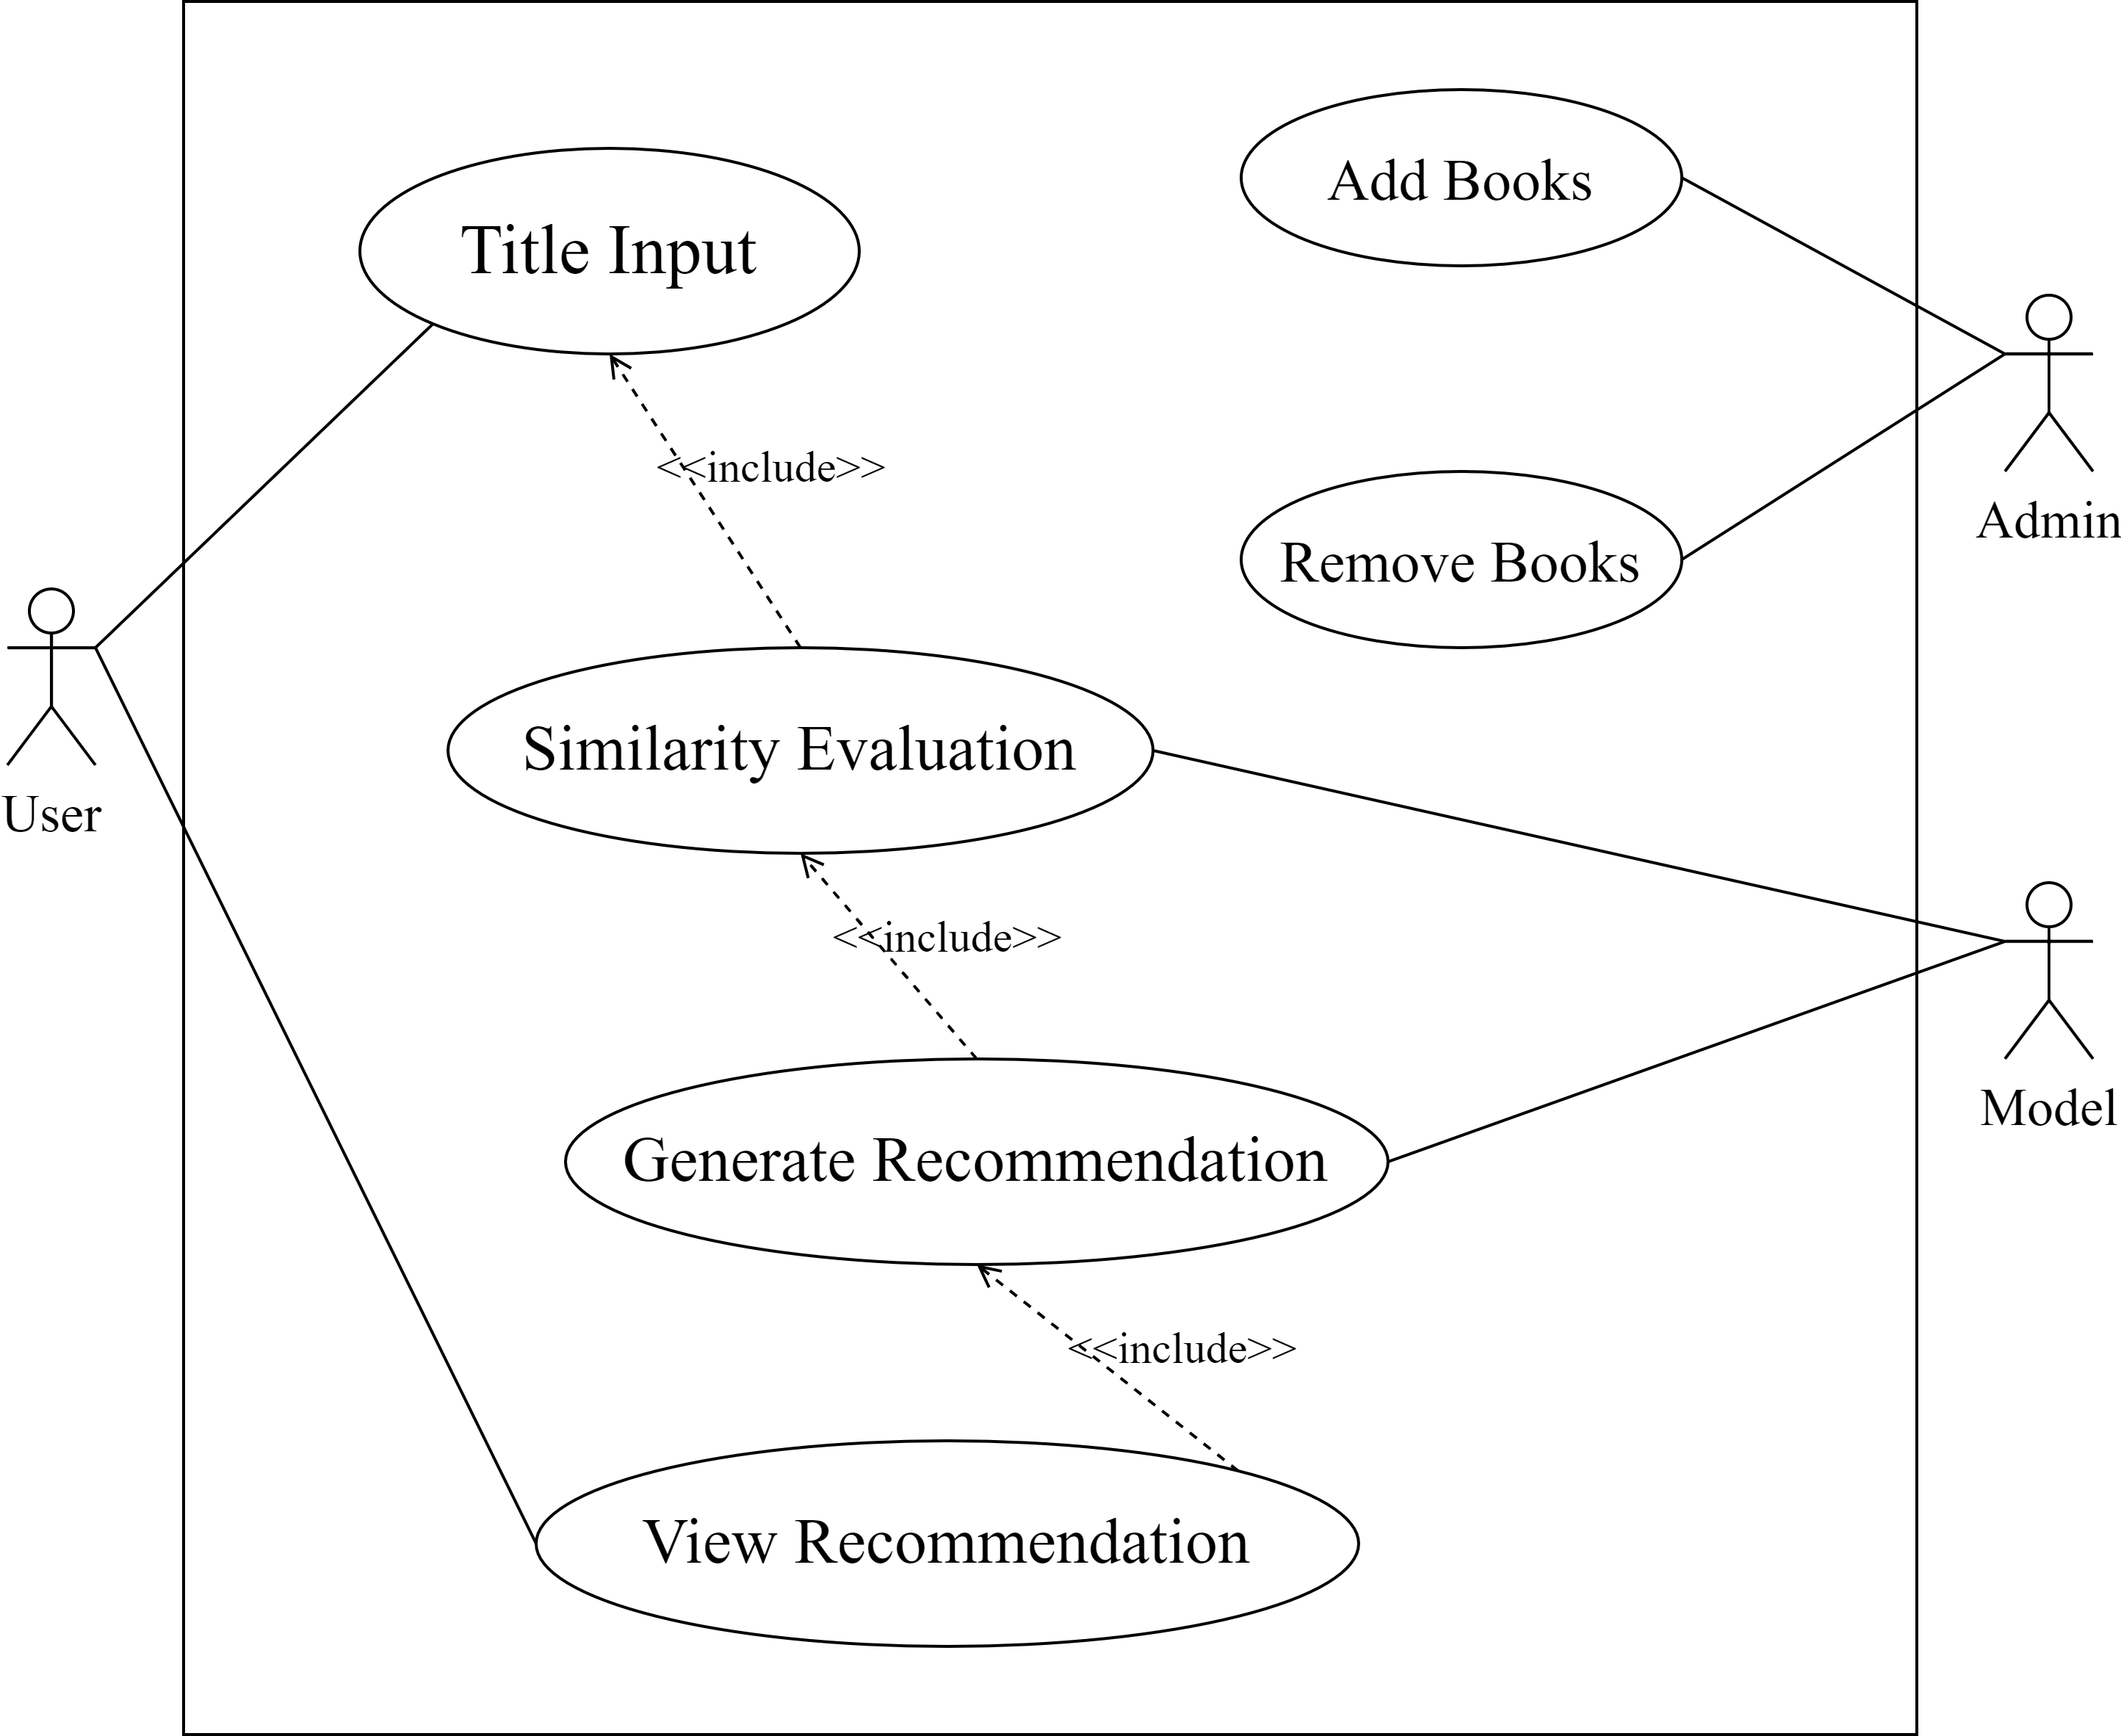
\includegraphics[width=1\linewidth, height=10cm]{img/Graphics/Use Case BRS.drawio.png}
    \caption{Use Case Diagram of Book Recommendation System}
    \label{Usecase}
\end{figure}
\newpage

\subsection{Class Diagram}
The class diagram for Book Recommendation System shows the various classes involved and the relationships among them.The diagram \ref{class-diagram} consists of the  following classes: User, Book, Model and Admin.
\begin{figure}[h]
    \centering
    \includegraphics[width=1\linewidth, height=10cm]{img/Graphics/classDiagram_BRS.png}
    \caption{Class Diagram of Book Recommendation System}
    \label{class-diagram}
\end{figure}
\subsection*{User Class}
Attributes\\
UserID: Unique identifier for each user.\\
Username: Name of the user.\\
Age: Age of the user.\\
Location: Location of the user.\\
Methods\\
giveRating(book): Allows the user to provide ratings for books.\\
searchBook(book): Enables the user to search for books based on various criteria.\\
viewRecommendation(book): Displays book recommendations for the user based on their preferences and ratings.\\

\subsection*{Book Class}
Attributes\\
ISBN: International Standard Book Number (ISBN) for each book.\\
bookName: Title of the book.\\
Author: Author(s) of the book.\\
Year of Publication: Year when the book was published.\\
Publisher: Publisher of the book.\\
Methods\\
getBookInfo(): Allows to view the information about book.\\
updateBookInfo(): Update the information about book.\\

\subsection*{Admin Class}
Attributes\\
adminID: Unique identifier for each admin.\\
Username: Name of the admin.\\
Methods\\
add\_remove(book): Allows the admin to add new books to the system and remove books from the system.\\
update(book): Allows the admin to update information about existing books.\\
manageUsers(user): Provides functionality for managing user accounts and permissions.\\

\subsection*{Model Class}
Attributes\\
modelID: Unique identifier for each recommendation model.\\
modelName: Name of the recommendation model.\\
Methods\\
get\_recommendation(book): Retrieves book recommendations using the KNN model.\\
evaluate\_model(): Evaluates the performance of the recommendation model based on various metrics.\\



\newpage
\subsection{Activity Diagram}
The activity diagram of Book recommendation system shows the flows
from the homepage of the web-app to the recommend system checks if the book is in database and provides recommendations in front UI if the book is present in database otherwise shows error. The diagram provides a comprehensive overview of the process involved in the recommendation engine, making it easier to understand the
entire workflow.
%\vspace{2cm}
\begin{figure}[h]
    \centering
    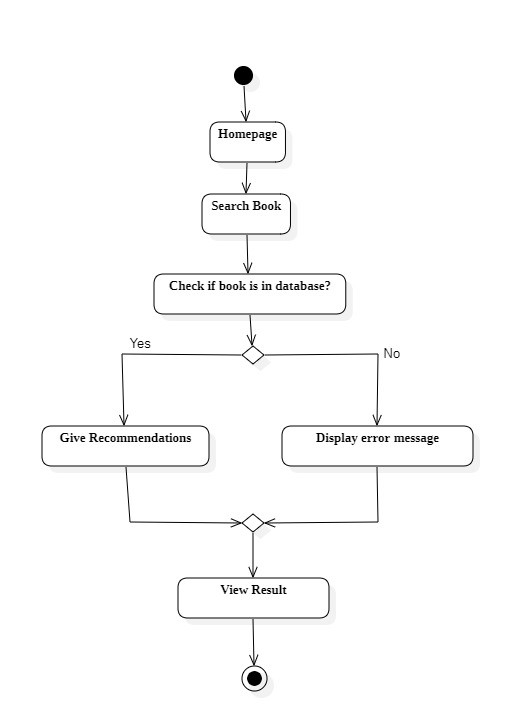
\includegraphics[width=0.9\linewidth]{img/Graphics/BRS_Activity.jpg}
    \caption{Activity Diagram for Book Recommendation System}
    \label{Activity}
\end{figure}
\newpage

\subsection{Sequence Diagram}
The sequence diagram shows the continuous flow of interaction between different part of system. The sequence diagram of book recommendation system shows the interactions between various components of the system such as user, user interface, backend server and database. To better visualize the behavior and interactions of the system, each step in the sequence stands for a particular action or message being passed between components. The user selects a book from the dropdown menu in webapp UI. The browser sends the selected book name to the backend server where the book name is checked in the book database and if found returns the recommendations for the given book by kNN model. The recommended books arrive back to the next page of the UI where there are details of the selected book along with it's recommendations. 
%\vspace{2cm}
\begin{figure}[h]
    \centering
    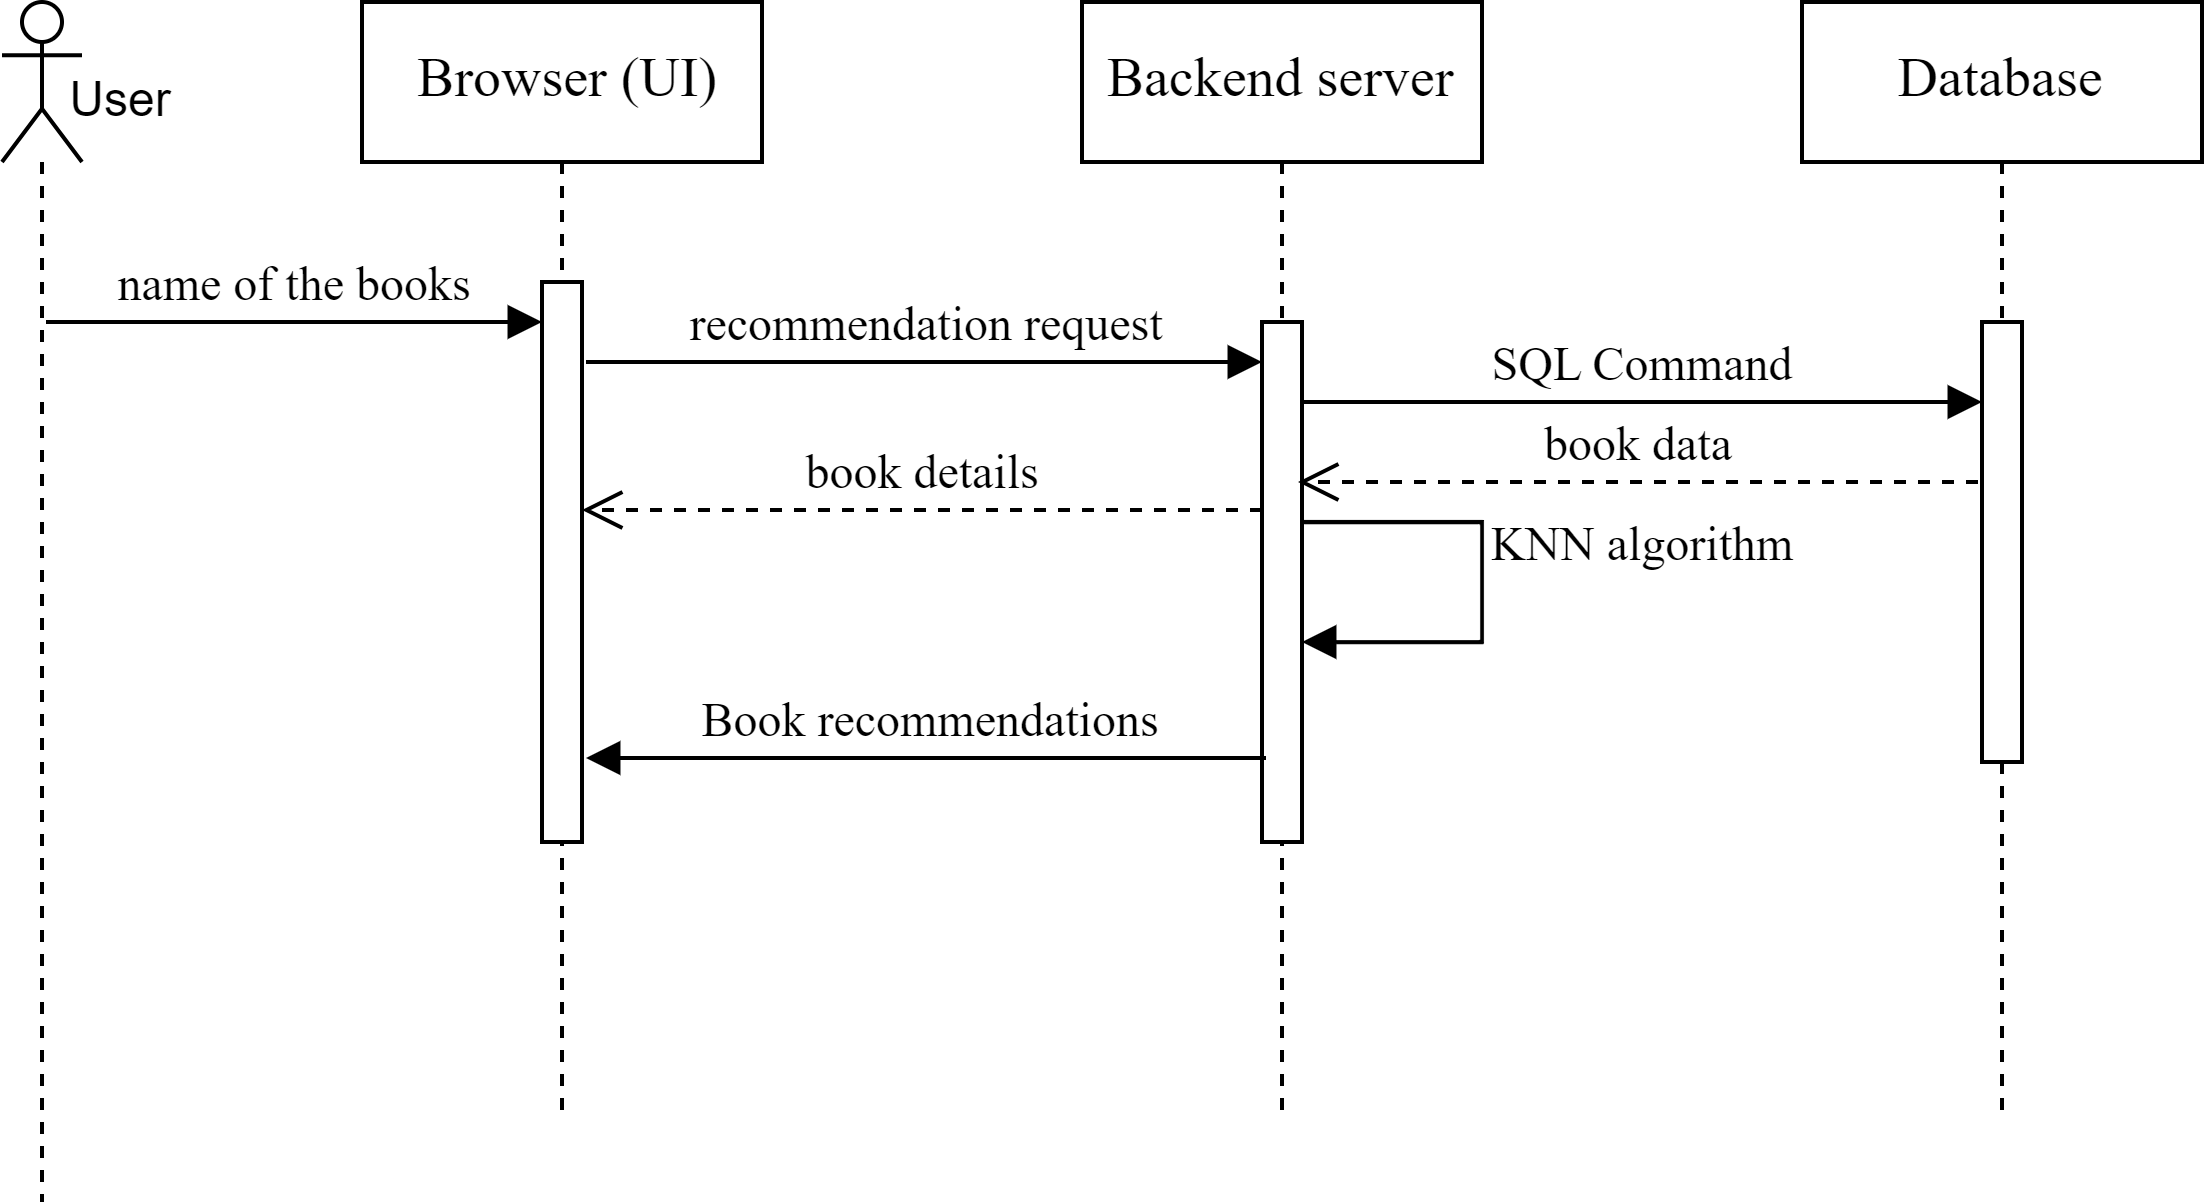
\includegraphics[width=1\linewidth]{img/Graphics/BRS_sequence.png}
    \caption{Sequence Diagram of Book Recommendation System }
    \label{Sequence}
\end{figure}
%\newpage

\subsection{ER Diagram}
The Entity Relationship (ER) diagram of Book Recommendation System shows the entities involved in the system, their attributes and the relationships between them. The entity relationship diagram of this system shows all the visual instrument of database tables and the relations between User, Book and Ratings. It is used to structure data and define the relationships between system structured data groups. The main entities of the system are User, Book and Ratings.

\subsection*{User}
This entity represents the users of the system.\\
Attributes\\ UserID: Primary Key (PK) uniquely identifying each user.\\
Age: The age provided by the user.\\
Location: The place of residence of the user.

\subsection*{Book}
This entity stores the details of books in the system.\\
Attribute\\ ISBN: Primary Key (PK) uniquely identifying each book.\\
BookName: The name of the book.\\
Author: The writer/creator of the book.\\
Publisher: The person/company behind distribution of the book.\\
BookImage: The picture of book cover generally front side.\\
YearofPublication: The date in which book launched.

\subsection*{Ratings}
This weak entity stores the ratings of books given by the users.\\
Attribute\\ UserID: Foreign Key (FK) uniquely identifying each user.\\
ISBN: Foreign Key (FK) uniquely identifying each book.\\
BookRatings: The ratings given to a book by a user.\\

 The relation between User and Book is one to many as one user can rate many books. Similarly, the relation between User and Ratings is also one to many because one user can give many ratings. The relation between Book and Ratings is also one to many as one book can have multiple ratings.
\vspace{2cm}
\begin{figure}[h]
    \centering
    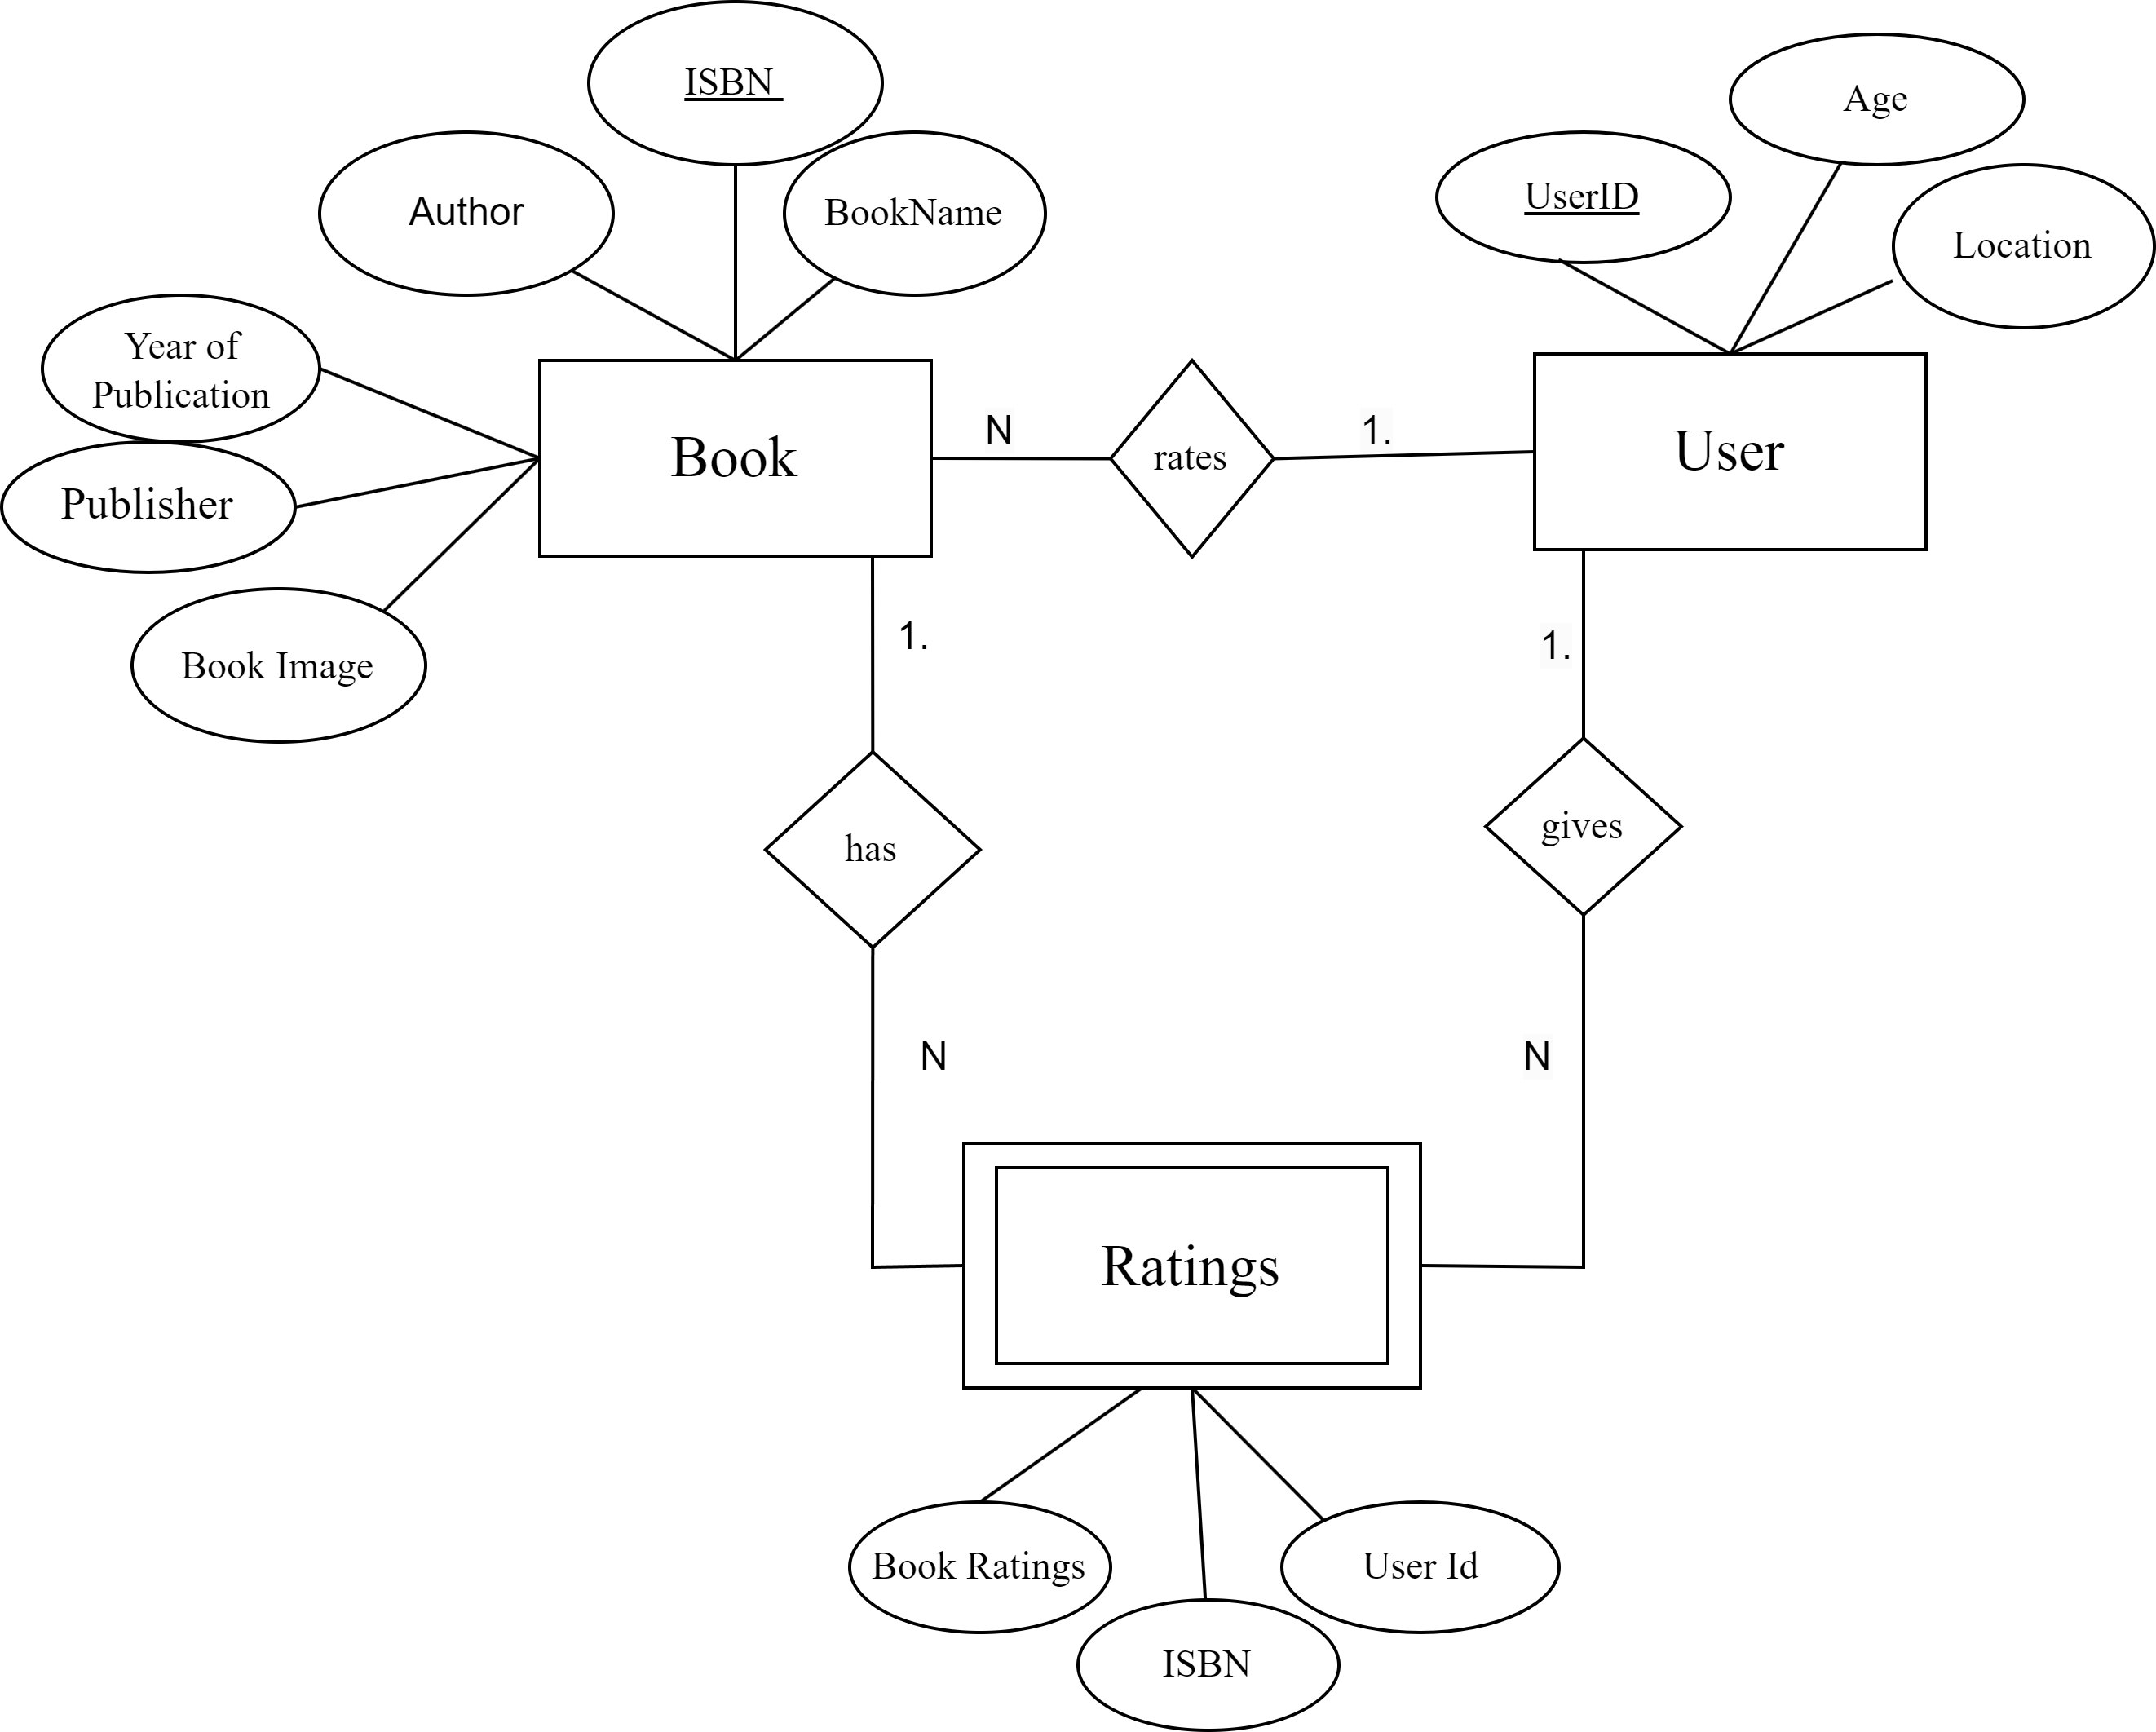
\includegraphics[width=1\linewidth]{img/Graphics/ER_brs.png}
    \caption{Entity Relationship Diagram}
    \label{Entity}
\end{figure}
\newpage

\subsection{DFD Level 0 Diagram}
The DFD level 0 diagram, also called context diagram of shows the high level overview of the whole system's interaction and functionalities. This diagram describes the system as a single process. This book recommendation system consists of three primary components: The User, Recommendation System and The Admin. The recommendation system is the main component that generate the recommendations to the user. Users interact with the system through user interface where users can search book with book name as input and the recommendation system process the input with the filtering technique and shows recommended books to the user. The admin update the dataset in the system and train the model using the revised data.
\vspace{2cm}
\begin{figure}[h]
    \centering
    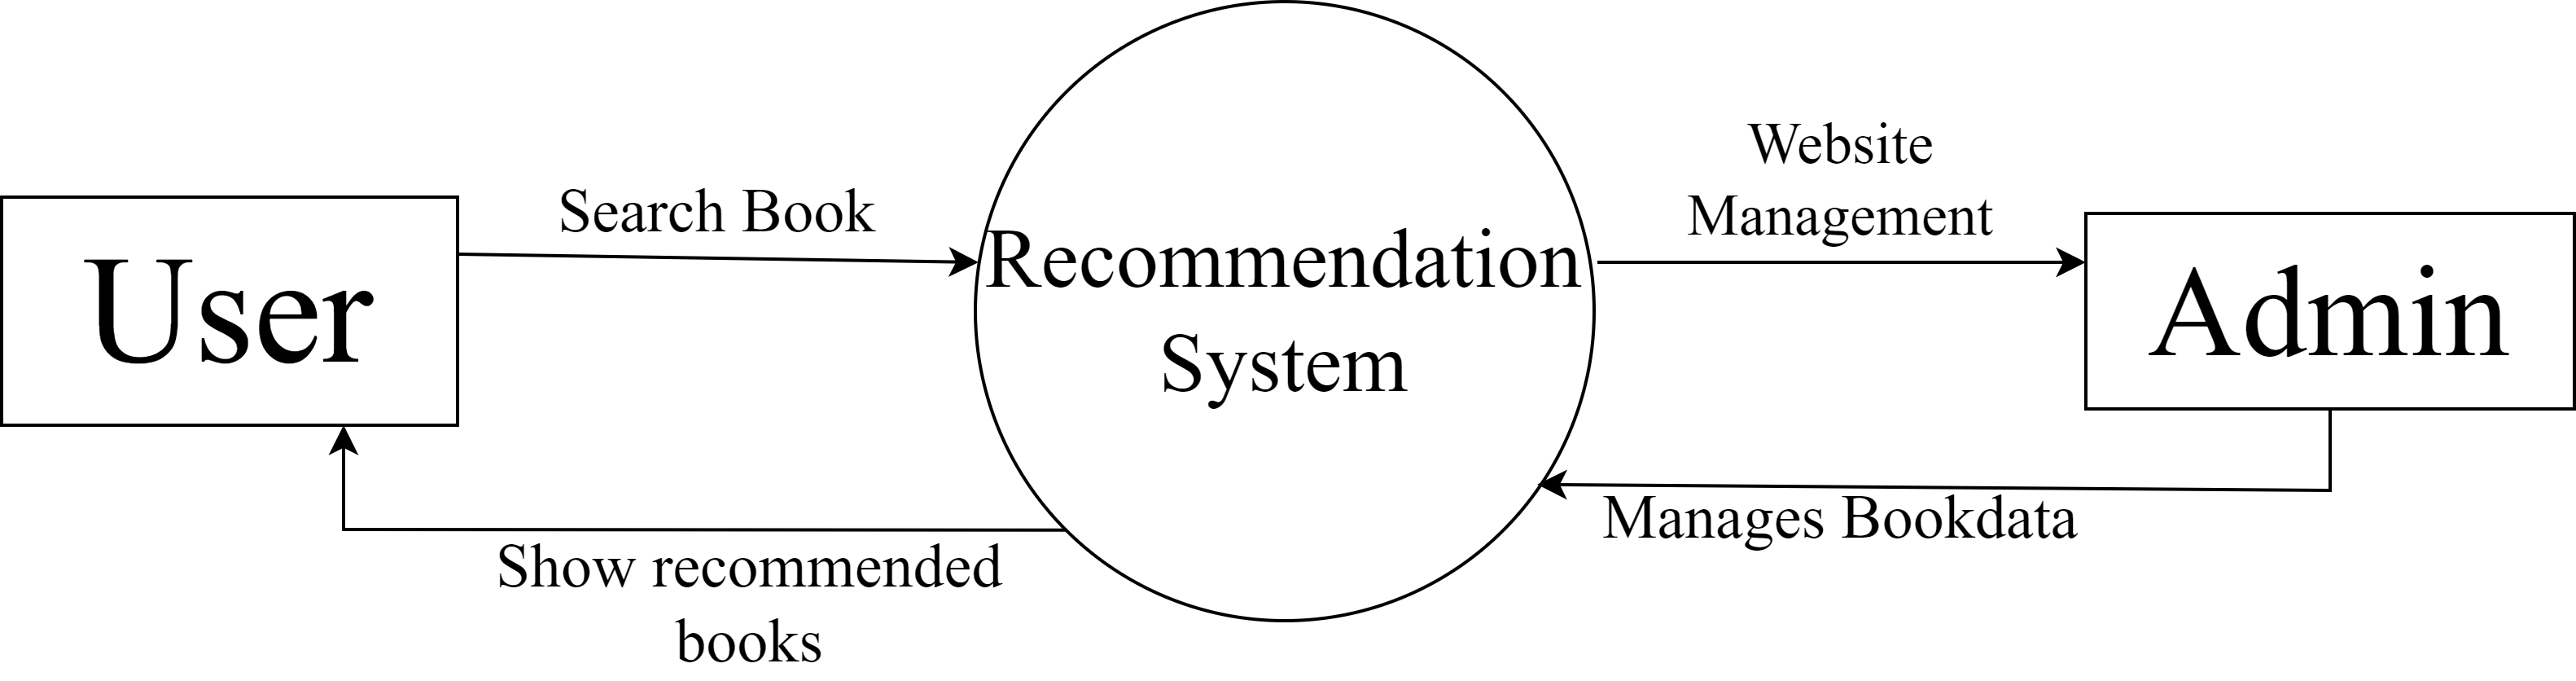
\includegraphics[width=1\linewidth]{img/Graphics/DFD_Level_0.drawio.png}
    \caption{DFD Level 0 Diagram}
    \label{DFD level 0}
\end{figure}
\newpage

\subsection{DFD Level 1 Diagram}
The DFD level 1 diagram shows the detailed view of the system by dividing the main process of the DFD level 0 into smaller processes. In DFD level 1, each sub-process is shown as a separate process and have their own specific function and task.Every sub-process in the DFD level 1 communicates with each other and the database through data flows. The transfer of information among processes, database and entities in the system is represents by there data flows. The book recommendation system's underlying procedures and how they interact to provide recommendations to users are depicted in greater detail and comprehensiveness in the Level 1 DFD. In the DFD level 1 diagram, the main component of the system recommendation system in further divided into different sub-processes. User search books with book name with the help of user interface and the system query in the book database. The book database is maintain by the admin. The system check if the book is available or not and if book is available, the recommendation engine receives the book details from the book database and it filter the book data on the basis of the model it is trained. The recommended books are shown to the user through the user interface.   
\vspace{1cm}
\begin{figure}[h]
    \centering
    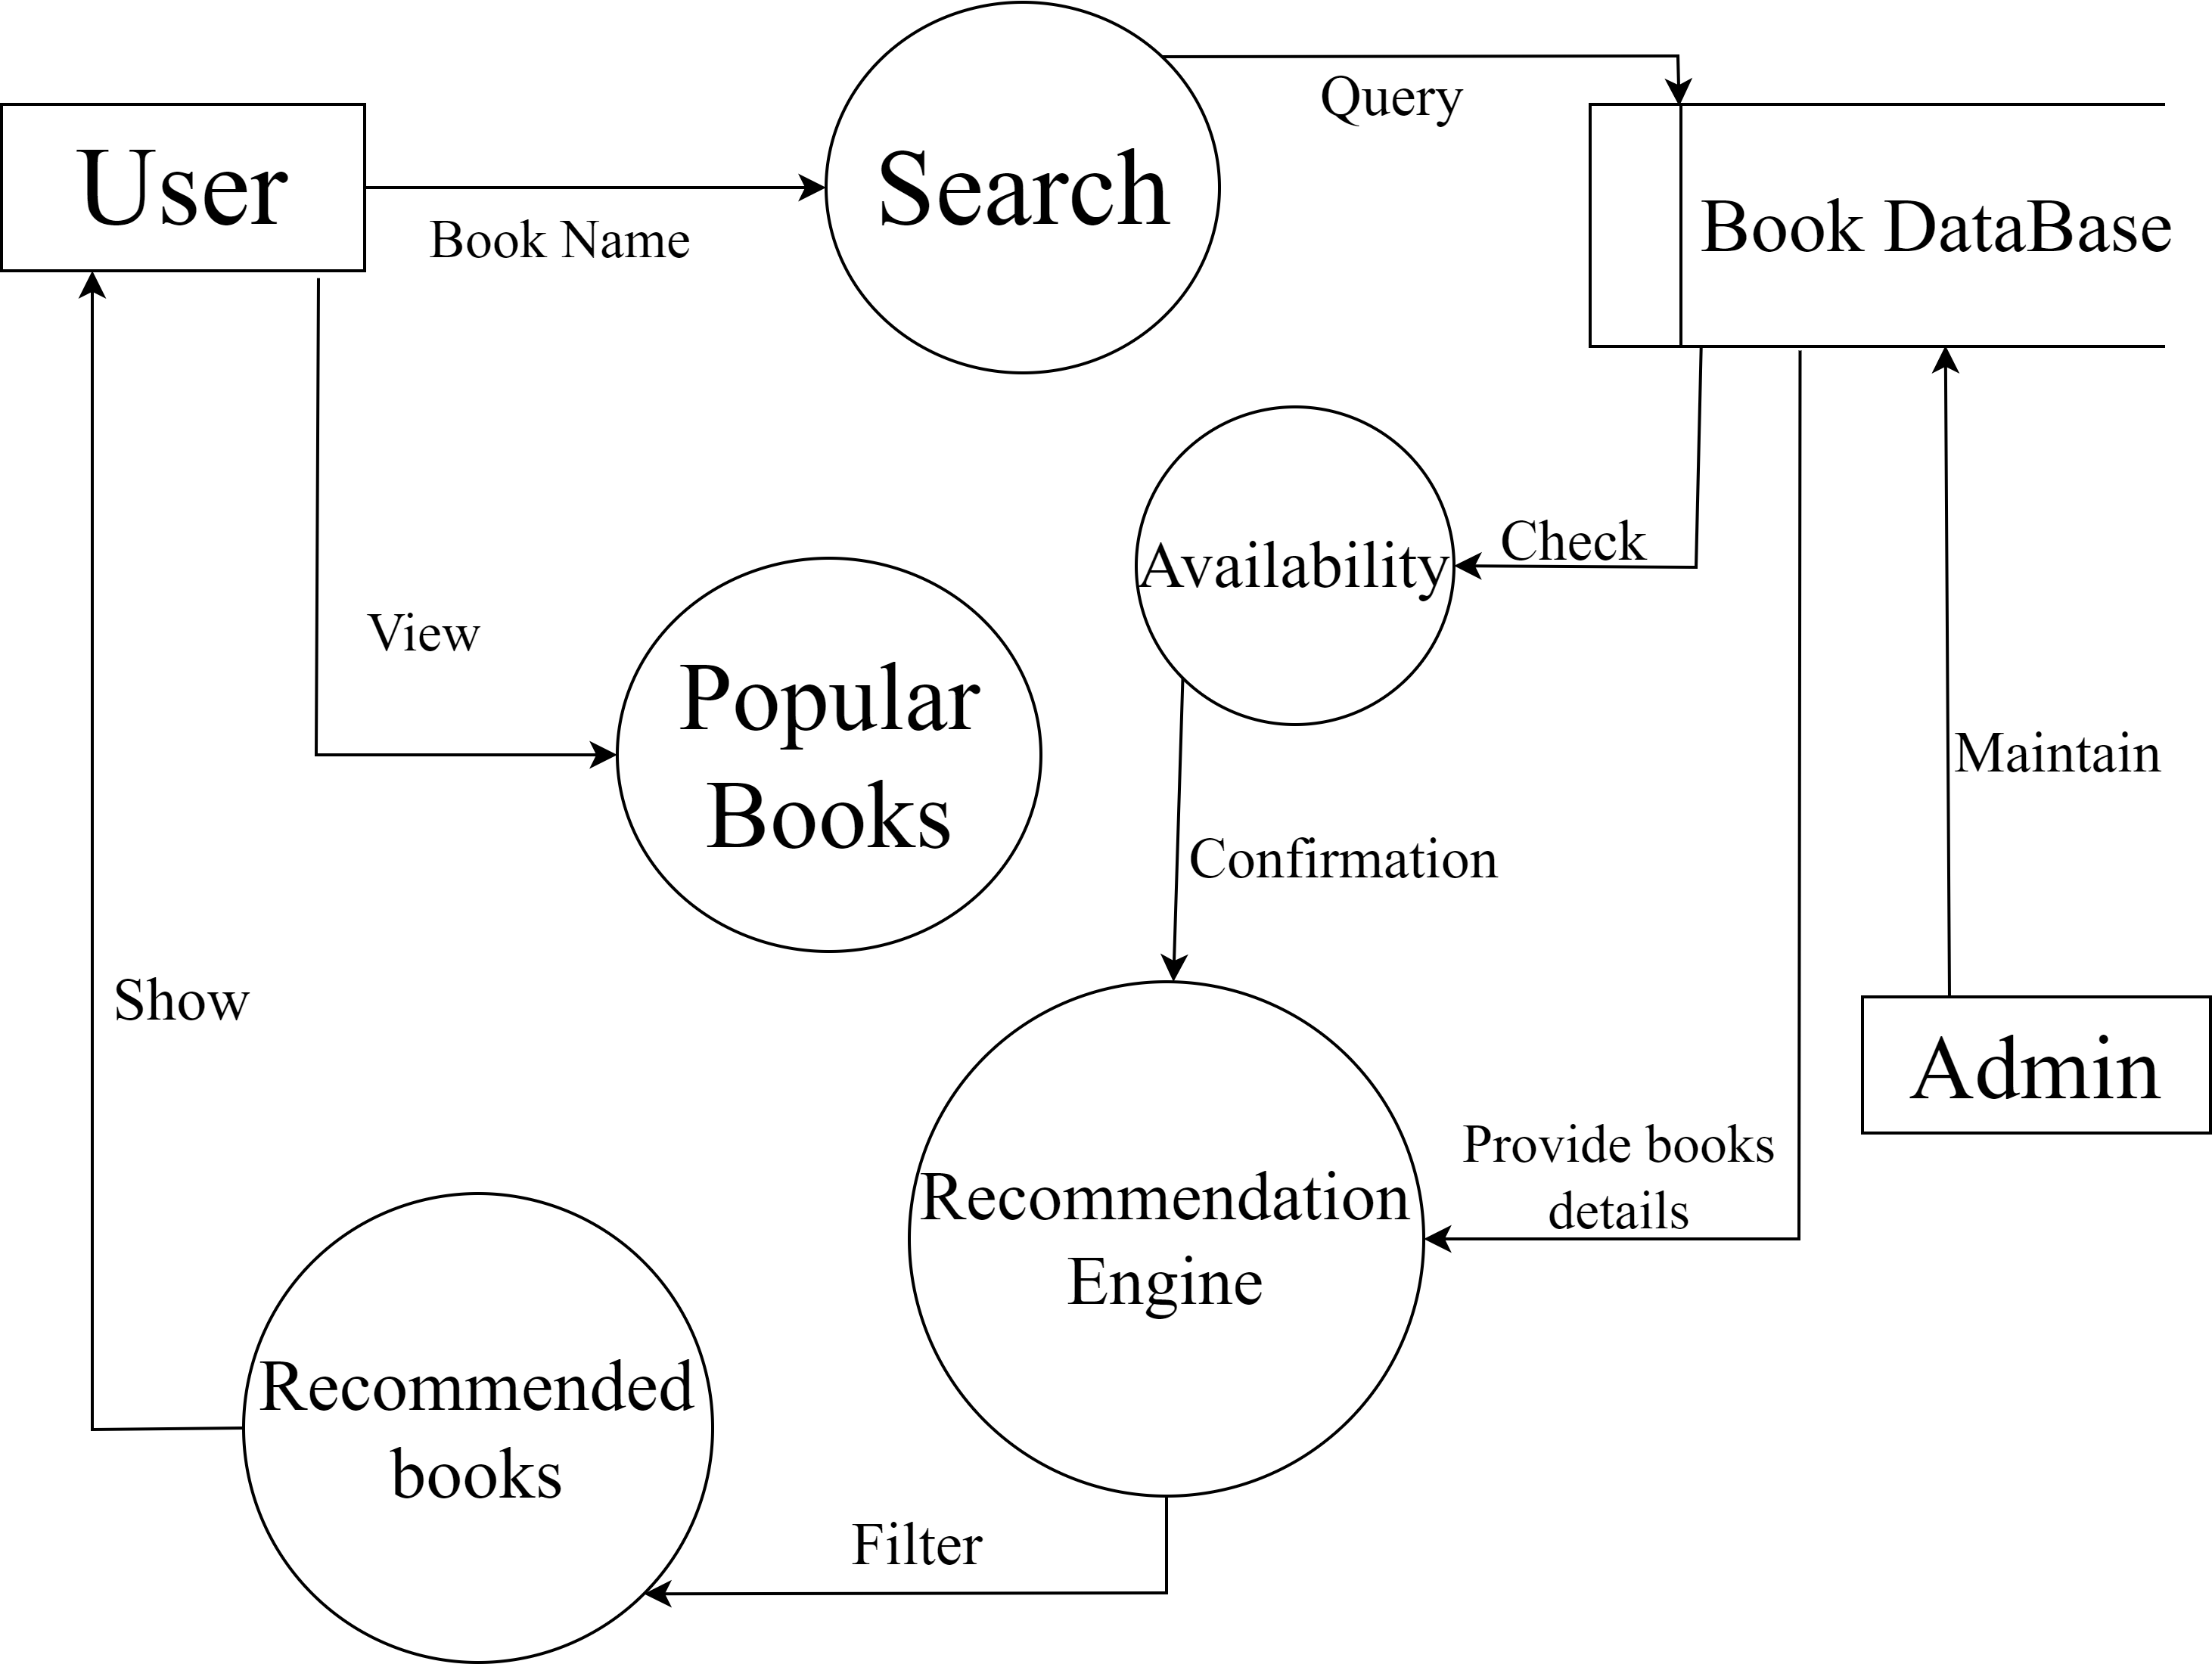
\includegraphics[width=1\linewidth]{img/Graphics/DFD_level_1.drawio.png}
    \caption{DFD Level 1 Diagram}
    \label{DFD level 1}
\end{figure}

\newpage
\section{Theoretical Formulations}

\subsection{Popularity Based Recommendations}
A popularity-based book recommendation system makes suggestions for books based on how well-liked they are overall among users, without taking individual user preferences into account. It is easy to use and doesn't need any user data, but it isn't personalised and might not provide a variety of suggestions. Popular books are determined by using the rating each books have got. By calculating the average rating of each book provided by the users and sorting the books with highest rating on top, popular book is determined and recommended. It works well in situations where readers are interested in popular, trending books or best sellers.

\subsection{Collaborative Filtering}
Collaborative filtering is a technique of filtering information and making automatic predictions by using the interactions and data collected by the system from the users. It works by matching the similarities in the items and users. It relies on user-item interactions, identifying patterns and preferences by analyzing user behaviors. The idea is simple, we frequently ask our friends for recommendations when we're looking for a new book to read. We trust recommendations from friends who have similar tastes to our own without a second thought. Let's use an example to better understand. A and B are two similar users, and A has read the books X, Y, and Z. The system will suggest X book to B user and W book to A user if B user had read Y, Z and W books. Two forms of collaborative filtering i.e item-based and user-based collaborative filtering has been analysed. In items-based collaboration, the similarity between items is the main focus of filtering, not users. Based on the preferences for similar items, the system will predict a user's preference for a particular item. And in user-based collaboration,a user will be recommended items that other users who share similar tastes have enjoyed.

\subsection{kNN Algorithm}
 KNN or k-nn, which stands for k-nearest neighbours algorithm, is an unsupervised learning algorithm based on regression that groups individual data points based on proximity in order to predict data. Although it can be applied to both classification or regression problems, it is used as a regression algorithm for recommendation systems, based on the idea that similar points can be located close to each other. Because it stores the dataset and acts on it when predicting, it is also known as a lazy learner algorithm. This is because it does not learn from the training set right away. It predicts a data point based on how its neighbours are classified.The K-NN algorithm predicts a new data point based on similarity after storing all the available data. This means that the K-NN algorithm can quickly predict newly discovered data into a well-suited category. K in KNN is a parameter that refers to the number of nearest neighbours to include in the majority voting process. The KNN algorithm uses the complete training dataset as a reference during the training phase. It uses a selected distance metric, such as Euclidean distance, to determine the distance between each training example and the input data point before making predictions. Based on their distances, the algorithm then determines the K closest neighbours of the input data point. The algorithm predicts the label for the input data point based on the most common class label among the K neighbours. For best results, careful parameter tuning is required as the choice of K and the distance metric can have an impact on the system's performance.

\subsection{Matrix Factorization Model}
A common technique in book recommendation systems is collaborative filtering, which involves matrix factorization as a fundamental operation. The aim of the matrix factorization model in a book recommendation system is to extract latent factors that represent user preferences and item characteristics by breaking down the user-item interaction matrix into lower-dimensional matrices. The model predicts user ratings for items they have not interacted with by learning these latent factors using optimisation algorithms like Singular Value Decomposition (SVD). The items with the highest predicted ratings are then suggested to users in recommendations that are generated based on the predicted ratings. All things considered, the model makes use of the connections that exist between users and books to offer precise and customised book recommendations.\\

\subsection{Dense Neural Network}
A Dense Neural Network (DNN) aka fully connected neural network is a type of neural network architecture composed of multiple layers, where each neuron in a layer is connected to every neuron in the subsequent layer.A DNN is typically composed of an input layer, one or more hidden layers and an output layer, where the parameters of the model include weights associated with each connections and the biases of each neurons.
The strength of dense neural networks in recommendation systems lies in their ability to learn and capture complex relationships between users, items, and other entities. They achieve this by utilizing dense vector representations (embeddings) of data, which unlike traditional data representation in form of sparse binary matrices, encode characteristics beyond simple presence or absence of interactions. These networks, with their multi-layered structure, can capture non-linear interactions between features. This allows them to consider various factors, such as how a user's past interactions with similar items influence their preferences for new recommendations, going beyond simple user-item correlations.
In essence, dense networks provide a powerful tool for recommendation systems by understanding the intricate connections within the data, leading to more accurate and personalized recommendations.


\subsection{Jaccard Similarity}

Jaccard similarity, also known as Jaccard index or Jaccard coefficient, is a metric used to compare the similarity between two sets. It measures the proportion of elements that are common to both sets relative to the total number of elements in the union of the two sets. The Jaccard similarity value ranges from 0 to 1, 0 meaning no elements being common to both sets and 1 meaning all elements common to both sets. Jaccards Similarity in context of recommendation system is used to identify users with similar tastes and suggest items based on shared preferences. It is used to compute User-Item Similarity or Item-Item similarity, hence measuring both similarity between users based on their past interactions with items (ratings) or similarity between items based on user interactions, enabling collaboration based recommendation in former case and content based recommendations in later. Jaccard similarity however treats all elements equally within a set and doesn't consider ratings of items to recommend which might lead to missing out on relevant items.


\section{Mathematical Modelling}

\subsection{Cosine Similarity}
By calculating the cosine of the angle between two vectors, as can be mathematically represented in equation, the cosine similarity method determines the similarity between two users. In cosine similarity, vectors represent the data objects in data sets, and the similarity is calculated and determined when they are defined in a product space as described in equation \ref{cosine}. 
\begin{equation}
\label{cosine}
Cosine-Similarity(A, B) = \frac{A.B}{||A||.||B||}
\end{equation}
Where\\
$\cdot$  represents the dot product of vectors. \\
$||\mathbf{A}||$  \text{ denotes the Euclidean norm (magnitude) of vector } $\mathbf{A}$. \\
$||\mathbf{B}|| $ \text{ denotes the Euclidean norm (magnitude) of vector } $\mathbf{B}$\\
The direction of a vector is determined by its angle, which is expressed in cos $\theta$ . The calculation of this angle  can be done using equation \ref{cosine}, which is equivalent to cos($||\mathbf{A}||$,$||\mathbf{B}||$). When $\theta$ = 0°, the “a” and “b” vectors overlap and prove to be similar. When $\theta$ = 90°, the “a” and “b” vectors are therefore dissimilar. \\ 
Let's consider two vectors \( \mathbf{A} \) and \( \mathbf{B} \):
\[ \mathbf{A} = \begin{pmatrix} 3 \\ 4 \\ 1 \end{pmatrix} \quad \text{and} \quad \mathbf{B} = \begin{pmatrix} 1 \\ 2 \\ 5 \end{pmatrix} \]
We can calculate the dot product of \( \mathbf{A} \) and \( \mathbf{B} \):
\[ \mathbf{A} \cdot \mathbf{B} = (3 \times 1) + (4 \times 2) + (1 \times 5) = 3 + 8 + 5 = 16 \]
Next, we compute the magnitudes (Euclidean norms) of \( \mathbf{A} \) and \( \mathbf{B} \):
\[ ||\mathbf{A}|| = \sqrt{3^2 + 4^2 + 1^2} = \sqrt{9 + 16 + 1} = \sqrt{26} \]
\[ ||\mathbf{B}|| = \sqrt{1^2 + 2^2 + 5^2} = \sqrt{1 + 4 + 25} = \sqrt{30} \]
Now, we can substitute these values into the cosine similarity formula:
\[ \text{Cosine Similarity}(\mathbf{A}, \mathbf{B}) = \frac{\mathbf{A} \cdot \mathbf{B}}{||\mathbf{A}|| \times ||\mathbf{B}||} = \frac{16}{\sqrt{26} \times \sqrt{30}} \]
Thus, the cosine similarity between \( \mathbf{A} \) and \( \mathbf{B} \) is:
\[ \text{Cosine Similarity}(\mathbf{A}, \mathbf{B}) = \frac{16}{\sqrt{26} \times \sqrt{30}} \approx 0.789 \]


\subsection{Matrix Factorization Model}
Consider a matrix R that represents the interactions between users and items, with users represented by rows and books by columns. Every entry \(r_{u,i}\) indicates the user u's rating and interaction with book i.
The user-item interaction matrix \(R\) is broken down into two lower-dimensional matrices by matrix factorization: one representing users \(U\) and the other representing items \(I\). Let \(U\) be an \(m \times k\) matrix where each row \(u_{i}\) represents the i\(-th\) user's latent factors. And \(I\) be an \(k \times n\) matrix, where each column \(i_{j}\) represents the j\(-th\) items latent factors. The objective is to identify matrices \(U\) and \(I\) in such a way that their product approximates the original user-item interaction matrix \(R\).
For a user \(u\) and item \(i\) the predicted rating \(\hat{r}_{u,i}\) is given by the dot product of the u\(-th\) row of \(U\) and the i\(-th\) column of \(I\) 
as described in equation \ref{MatFact}.
\begin{equation}
\label{MatFact}
\hat{r}_{u,i} = u_i \cdot i_j
\end{equation}
Consider the matrices $U$ and $I$ as follows:
\[ U = \begin{pmatrix}
1 & 0.5 \\
0.8 & 0.2 \\
0.6 & 0.3 \\
\end{pmatrix} \]
\[ I = \begin{pmatrix}
0.9 & 0.6 & 0.3 \\
0.7 & 0.4 & 0.2 \\
\end{pmatrix} \]
Let's calculate the predicted rating $\hat{r}_{2,3}$ for user $2$ and item $3$ using equation (4.2).
\[ \hat{r}_{2,3} = u_2 \cdot i_3 \]
\[ \hat{r}_{2,3} = (0.8 \ 0.2) \cdot \begin{pmatrix} 0.3 \\ 0.2 \end{pmatrix} \]
\[ \hat{r}_{2,3} = (0.8 \times 0.3) + (0.2 \times 0.2) \]
\[ \hat{r}_{2,3} = 0.24 + 0.04 \]
\[ \hat{r}_{2,3} = 0.28 \]
So, the predicted rating for user $2$ and item $3$ is $0.28$.

\subsection{Euclidean Distance}
Euclidean distance is a distance metric that is frequently used in the k-NearestNeighbours (KNN) algorithm to determine how similar two data points are to one another. The main idea behind KNN is to use the average value or majority label of a data point's k-nearest neighbours in the feature space to predict the label or value of a new data point.
For each data point in the dataset, calculate the Euclidean distance to the new data point (the one you want to classify or predict) as shown in equation \ref{euclidist}.
\begin{equation}
\label{euclidist}
Euclidean-Distance(P, Q) = \sqrt{{\sum_{i=1}^{n} (p_i - q_i)^2}}
\end{equation}

Where\begin{align*}
    P & = (p_1, p_2, \ldots, p_n) \\
    Q & = (q_1, q_2, \ldots, q_n)
\end{align*}
are the coordinates of the two points in \(n\)-dimensional space. \(p_i\) and \(q_i\) represent the \(i\)-th dimension of points \(P\) and \(Q\), respectively.\\
Let's consider two vectors $P$ and $Q$ with random data:
\[
P = (3, 1, 2, 5, 4) \quad \text{and} \quad Q = (1, 2, 3, 2, 5)
\]
The Euclidean distance between $P$ and $Q$, denoted as $d(P, Q)$, is calculated using formula (4.3):
\[
d(P, Q) = \sqrt{\sum_{i=1}^{5} (p_i - q_i)^2}
\]
Substituting the given values:
\[
d(P, Q) = \sqrt{(3 - 1)^2 + (1 - 2)^2 + (2 - 3)^2 + (5 - 2)^2 + (4 - 5)^2}
\]
\[
d(P, Q) = \sqrt{2^2 + (-1)^2 + (-1)^2 + 3^2 + (-1)^2}
\]
\[
d(P, Q) = \sqrt{4 + 1 + 1 + 9 + 1}
\]
\[
d(P, Q) = \sqrt{16} = 4
\]
So, the Euclidean distance between vectors $P$ and $Q$ is $4$.


\subsection{Jaccard Similarity}
Jaccard similarity index is a metric used to compare the similarity and dissimilarity between two sets. It can be expressed as the ratio of the size of the sets' union and the size of their intersection. The mathematical formula for calculating Jaccard similarity index is shown in equation \ref{jaccard}
\begin{equation}
\label{jaccard}
J(A, B) = \frac{|A \cap B|}{|A \cup B|}
\end{equation}
Where:\\
\( A \) and \( B \) are sets being compared.\\
\( |A \cap B| \) denotes the number of elements(items/users) shared between both sets \( A \) and \( B \) (the size of the intersection).\\
\( |A \cup B| \) denotes the total number of elements(items/users) in sets \( A \) and \( B \) combined (the size of the union).\\
Let's calculate $J(A, B)$ for two sample sets:

Let $A = \{1, 2, 3, 4\}$ and $B = \{3, 4, 5, 6\}$.

The intersection of sets $A$ and $B$, $|A \cap B|$, is $\{3, 4\}$, and the union of sets $A$ and $B$, $|A \cup B|$, is $\{1, 2, 3, 4, 5, 6\}$.

Therefore,

\[
J(A, B) = \frac{|\{3, 4\}|}{|\{1, 2, 3, 4, 5, 6\}|} = \frac{2}{6} = \frac{1}{3}
\]

So, the Jaccard similarity coefficient between sets $A$ and $B$ is $\frac{1}{3}$.





%\section{Verification and Validation Procedures}
